Please draw the vector $\boldsymbol{w} = \boldsymbol{Av}$ where $\boldsymbol{A}$ is

\begin{align*}
    \boldsymbol{A} = \begin{bmatrix}
    \frac{1}{\sqrt{2}} & -\frac{1}{\sqrt{2}} \\
    \frac{1}{\sqrt{2}} & \frac{1}{\sqrt{2}}
    \end{bmatrix}
\end{align*}

\begin{solution}
\begin{align*}
    \boldsymbol{w} = \boldsymbol{Av} = \begin{bmatrix}
    \frac{1}{\sqrt{2}} \\ \frac{1}{\sqrt{2}}
    \end{bmatrix}
\end{align*}

\begin{center}
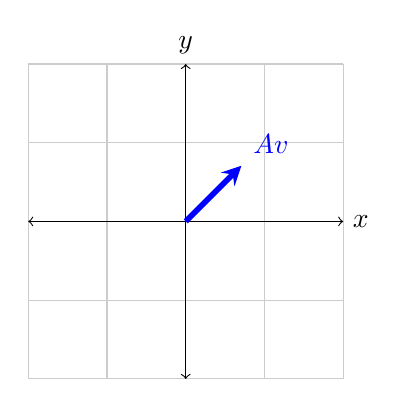
\begin{tikzpicture}
  \draw[thin,gray!40] (-2,-2) grid (2,2);
  \draw[<->] (-2,0)--(2,0) node[right]{$x$};
  \draw[<->] (0,-2)--(0,2) node[above]{$y$};
  \draw[line width=2pt,blue,-stealth](0,0)--(0.707,0.707) node[anchor=south west]{$\boldsymbol{Av}$};
\end{tikzpicture}
\end{center}
\end{solution}